\documentclass[portugues]{beamer}
\usepackage[T1]{fontenc}
\usepackage[utf8]{inputenc}
\usepackage[portuges]{babel}

\usepackage{amsmath}
\usepackage{amsfonts}
\usepackage{mathtools}
\usepackage{verbatim}
\usepackage{float}
\usepackage{graphicx}
\usepackage{times}  

\usepackage{array}
\usepackage{makecell}
\usepackage{tikz}
\usepackage{amsthm}
\usepackage{lscape}
%\usepackage[lined, boxed, linesnumbered]{algorithm2e}
%\usepackage{color}
\usetheme{Dresden}

\setbeamertemplate{headline}{\scriptsize{\vspace*{0.3cm}\hspace*{0.3cm}\insertframenumber}} 

\begin{document}
\title{VNE-AC: Virtual Network Embedding Algorithm Based on Ant Colony Metaheuristic}
\author{Leonardo Moura}

%\date{December 21, 2012} 

\frame{\titlepage \thispagestyle{empty}} 

\frame{\frametitle{Sumário}\tableofcontents \thispagestyle{empty}} 

\section{Introdução} 

\frame{\frametitle{O Artigo}
\setcounter{framenumber}{1}
\begin{itemize}
      \item 2011 IEEE International Conference on Communications (ICC)
      \item \textbf{Índice H}: 53
      \item \textbf{Qualis}: A2
      \item \textbf{Google}: citado por 23
      \item \textbf{IEEEXPLORE}: citado por 5
\end{itemize}
}

\frame{\frametitle{Mapeamento de Redes Virtuais}
Consiste em rodar múltiplas redes virtuais no mesmo substrato físico. Redes virtuais vêm sendo reconhecidas como a solução para o problema de estagnação dos protocolos da Internet. Também pode ser usado academicamente para teste de novos protocolos.
  }
  % -----------------------------------------------------------------------------
  \section{O Problema}
  \frame{\frametitle{Instância do Problema}
  \begin{columns}[c]
    \column{.5\textwidth}
      \begin{figure}[h]
        \centering
        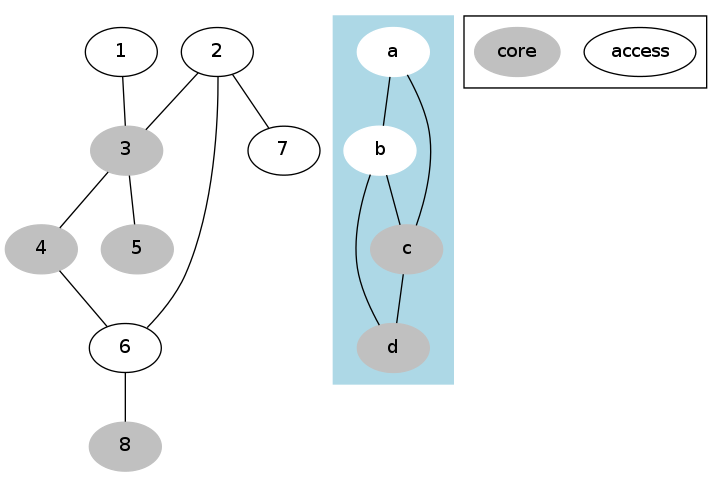
\includegraphics[scale=0.30]{g1.png}
      \end{figure}
     \column{.5\textwidth}
       Cada vértice: CPU, memória, localização e tipo.
       Nodos de acesso são aqueles em que o tráfego entra ou sai da rede
       Cada link: banda.
   \end{columns}
  }

  \frame{\frametitle{Exemplo de Solução}
  \begin{figure}[h]
    \centering
    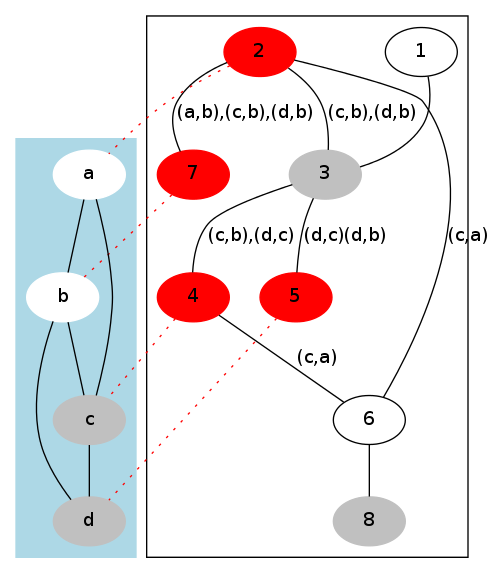
\includegraphics[scale=0.30]{gfinal.png}
  \end{figure}
  }

  % -----------------------------------------------------------------------------
  \section{O Algoritmo, Max Min Ant Colony System}
  \frame{\frametitle{Max Min Ant Colony System}
  \begin{columns}
    \column{.3\textwidth}
      \begin{figure}[h]
        \centering
        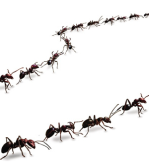
\includegraphics[scale=0.60]{ants.png}
      \end{figure}
    \column{.7\textwidth}
      \begin{itemize}
        \item Baseado na natureza;
        \item Diversificação: Valores de feromônio começam elevados;
        \item Intensificação: Após várias iterações, os mapeamentos que levam a melhores soluções vão ter maior probabilidade de serem selecionados.
    \end{itemize}
\end{columns}
}

\frame{\frametitle{Primeira Fase: Mapeamento dos nodos de acesso}
\begin{figure}[h]
  \centering
  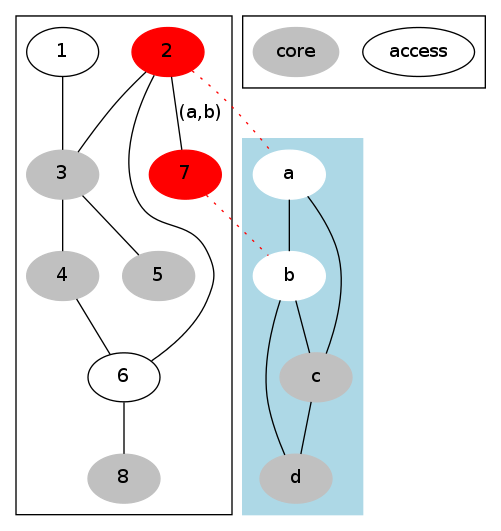
\includegraphics[scale=0.30]{g2.png}
\end{figure}
}

\frame{\frametitle{Geração dos componentes}
\begin{figure}[h]
  \centering
  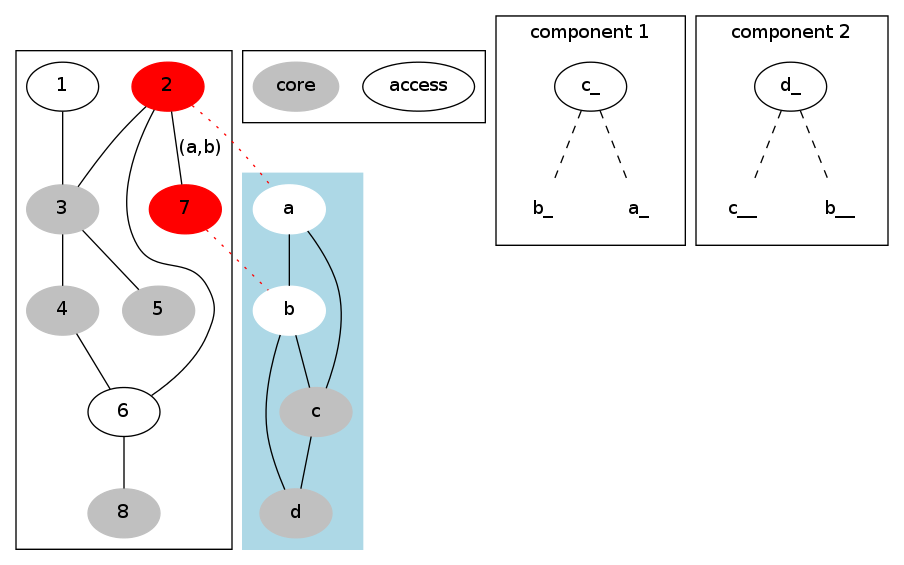
\includegraphics[scale=0.30]{g3.png}
\end{figure}
}

\frame{\frametitle{Candidatos para cada Componente}
\begin{figure}[h]
  \centering
  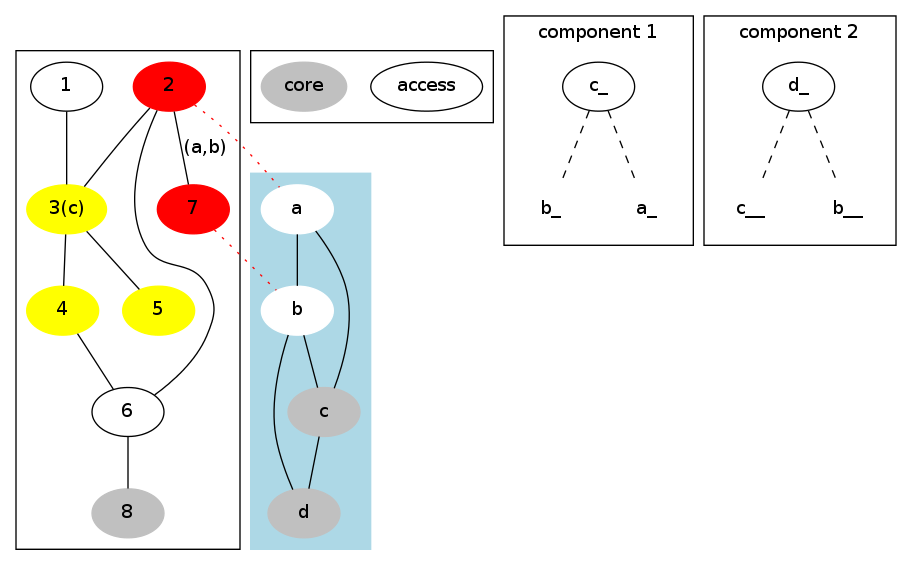
\includegraphics[scale=0.30]{g4.png}
\end{figure}

%Candidatos: H hops do baricentro.
}

\frame{\frametitle{Mapeamento de um Componente}
\begin{equation}
  p_{ab} = \frac{\tau^{\alpha}_{ab} \eta^{\beta}_{ab}}
  {\sum_{b \in PN_{a}} \tau^{\alpha}_{ab} \eta^{\beta}_{ab}}
\end{equation}
}

\frame{\frametitle{Mapeamento de um dado Componente por uma Formiga}
\begin{figure}[h]
  \centering
  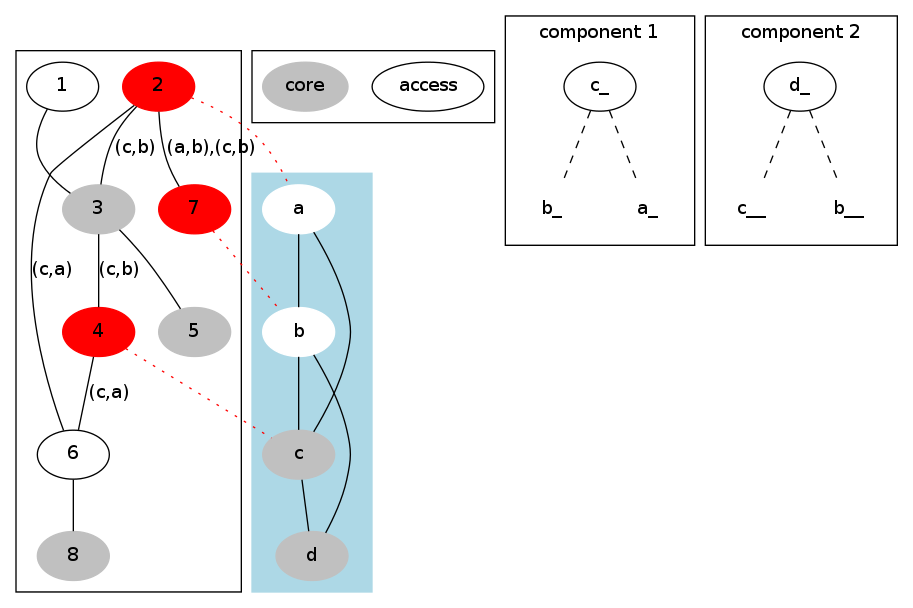
\includegraphics[scale=0.30]{g5.png}
\end{figure}
}

\frame{\frametitle{Mapeamento de um Link}
\begin{figure}[h]
  \centering
  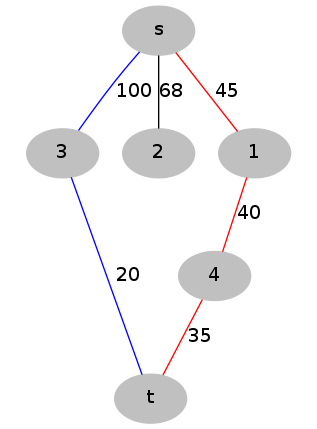
\includegraphics[scale=0.30]{gpathraw.png}
\end{figure}
}

\frame{\frametitle{Algoritmo de Dijkstra}
\begin{columns}[c]
  \column{.5\textwidth}
\begin{figure}[h]
  \centering
  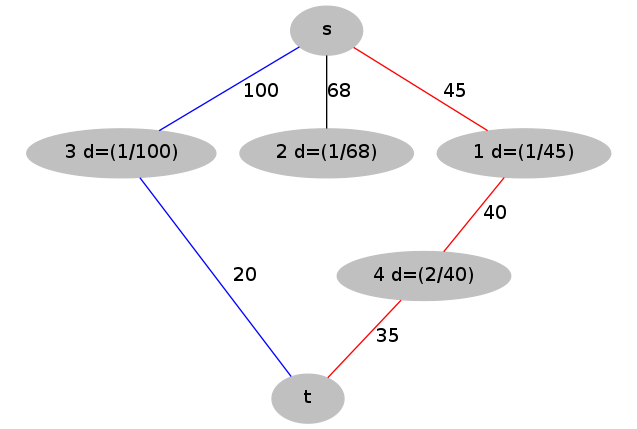
\includegraphics[scale=0.30]{gpath.png}
\end{figure}
  \column{.5\textwidth}
\begin{equation}
  d(P) = \frac{lenght(P)}{\min_{e^{S}_{x}\in P}B_{e^{S}_{x}}}\label{metric}
\end{equation}
\end{columns}
}

\frame{\frametitle{Reforço do Feromônio}
\begin{equation}
  \tau_{ab}(t+1) = \left\{  
  \begin{array}{l l}
    \rho \tau_{ab}(t) + \frac{\phi}{best solution cost} & \text{if $a$ was mapped to $b$ in the}\\
                                                        & \text{best solution of iteration $t$} \\
    \rho \tau_{ab}(t) & \text{otherwise}
  \end{array}\right .
\end{equation}
}

\frame{\frametitle{Trabalho Realizado}
\begin{itemize}
  \item Gerador de Instâncias (GT-ITM tool)
  \item Programa de Mapeamento
  \item Verificador
  \item Simulador de requisições
\end{itemize}
}

\frame{\frametitle{Informações Não Encontradas}
\begin{itemize}
  \item Processo de seleção dos parâmetros
  \item Parâmetros: $\tau_{min}, \tau_{max}, \phi, \rho$
  \item Forma de atribuir o tipo acesso ou core para nodos
  \item Qual a relação entre as redes virtuais, o que significa o tempo de vida
\end{itemize}
}
% -----------------------------------------------------------------------------
\section{Resultados Experimentais}

\frame{\frametitle{Simulação}
\begin{columns}[c]
  \column{.6\textwidth}
\begin{figure}[h]
  \centering
  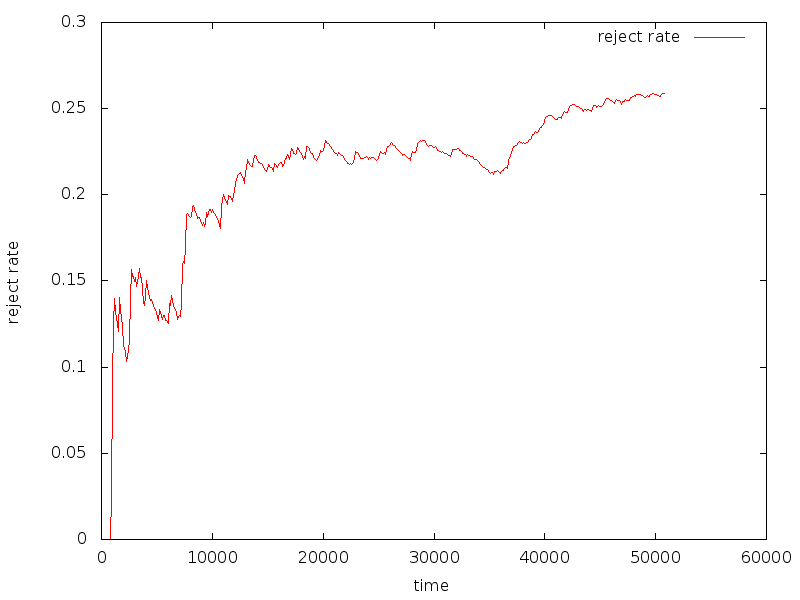
\includegraphics[scale=0.20]{rejectrate.png}
  \caption{Tempo x Taxa de Rejeição}
\end{figure}
  \column{.4\textwidth}
  \begin{itemize}
    \item Simulação com 4 requisições em média por 100 unidades de tempo
    \item Cada requisição com tempo de vida exponencial com média 1000
    \item Simulação sobre 2000 requisições
  \end{itemize}
\end{columns}
}

\frame{\frametitle{}
\begin{figure}[h]
  \centering
  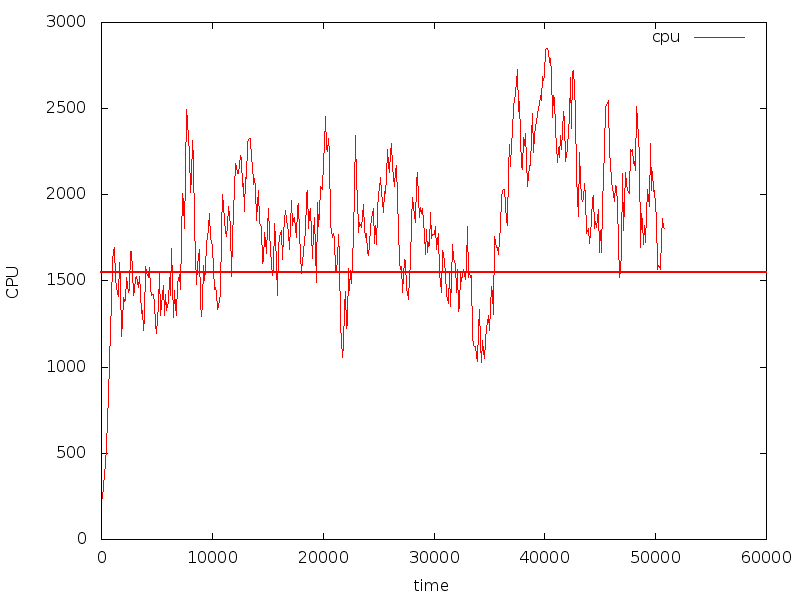
\includegraphics[scale=0.30]{cpu.png}
  \caption{Limitante Inferior na quantidade de cpu nos nodos de acesso necessária para aceitar todas as requisições}
\end{figure}
}

% -----------------------------------------------------------------------------
\section{Conclusão}
\frame{\frametitle{Conclusão} 
\begin{itemize}
  \item Problema e Solução Interessantes
  \item Importância de informar todos os parâmetros e requisitos
  \item Sugestão de mapeamento aleatório também dos nodos de acesso (que são mapeados gulosamente)
\end{itemize}
}

\frame{\vspace{0.15\textheight}
  {\huge Muito Obrigado}
  
\begin{figure}[h]
  \centering
  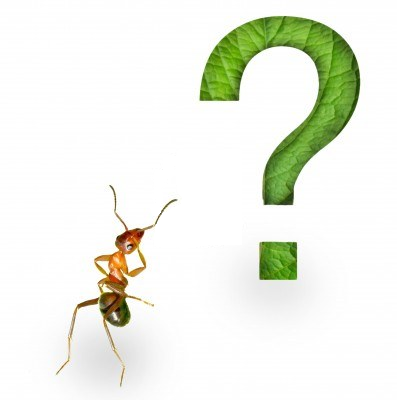
\includegraphics[scale=0.60]{questionant.png}
\end{figure}
}

\end{document}
